\documentclass[a4paper,10pt]{article}
\usepackage[utf8]{inputenc}
\usepackage{graphicx}
\usepackage{url}
\usepackage{float}
\usepackage{times}
\usepackage{multirow}
\usepackage{listings}
\usepackage{times}
\usepackage{paralist}
\usepackage{epsfig}
\usepackage{subfigure}
\usepackage[hypertex]{hyperref}
\usepackage{subfigure}
\usepackage{color}
\usepackage{xspace}

%\documentclass{rspublic}

\usepackage{ifpdf}

\newcommand{\I}[1]{\textit{#1}}
\newcommand{\B}[1]{\textbf{#1}}
\newcommand{\BI}[1]{\textbf{\textit{#1}}}
\newcommand{\T}[1]{\texttt{#1}}

\newcommand{\sagaspec}{\textit{SAGA}\xspace}
\newcommand{\sagaimpl}{\textit{SAGA}\xspace}

\newcommand{\spec}{\sagaspec}
\newcommand{\impl}{\sagaimpl}

\setlength\topmargin{0in}
\setlength\headheight{0in}
\setlength\headsep{0in}
\setlength\textheight{9.5in}
\setlength\textwidth{6.5in}
\setlength\oddsidemargin{0in}
\setlength\evensidemargin{0in}
\setlength\parindent{0.1in}
\setlength\parskip{0.25em}


\ifpdf
 \DeclareGraphicsExtensions{.pdf, .jpg}
\else
 \DeclareGraphicsExtensions{.eps, .ps}
\fi

\newcommand{\note}[1]{ {\textcolor{red} { ***NOTE: #1 }}}

\newif\ifdraft
\drafttrue

\ifdraft
\newcommand{\amnote}[1]{   {\textcolor{magenta} { ***Andre:    #1 }}}
\newcommand{\jhanote}[1]{  {\textcolor{red}     { ***Shantenu: #1 }}}
\newcommand{\onote}[1]{  {\textcolor{blue}     { ***Ole: #1 }}}
\else
\newcommand{\amnote}[1]{}
\newcommand{\jhanote}[1]{}
\newcommand{\onote}[1]{}
\fi

\begin{document}

 \title{ \large \vspace{-3.5em} SAGA: Towards a Comprehensive
   Programming System for Distributed Scientific Applications }
 \jhanote{We should discuss the title. I'm not a 100\% comfortable}
 
 \onote{What about: \textit{SAGA: Towards a Practical Programming System...} (i.e. SAGA is not 
 comprehensive). Or what about: \textit{SAGA: An Applied Approach Towards a
   Programming System for Distributed Scientific Applications}}

 
 \author{\normalsize Ole Weidner$^{1,3}$, Andre Merzky$^{1}$, Hartmut Kaiser$^{1}$, Shantenu Jha$^{1,2,4}$\\
   \small{\emph{$^{1}$Center for Computation \& Technology, Louisiana State University, USA}}\\
   \small{\emph{$^{2}$Department of Computer Science, Louisiana State University, USA}}\\
   \small{\emph{$^{3}$School of Informatics, University of Edinburgh, UK}}\\
   \small{\emph{$^{4}$e-Science Institute, University of Edinburgh, UK}}
 }
 \date{}
 \maketitle
 

% \jhanote{Remember in addition to serving as an abstract, this will
%   serve as a summary of what will go to the 3 editors of the journals
%   that we are considering publishing a full paper in. Thus some more
%   information/discussion on what the underlying problem and context
%   will be about.}


% \jhanote{Once we have defined / introduced SAGA, we should probably
%   have 3 subsections -- interface, library and adatptors/backends?}

\subsection*{Abstract}
%\vspace{-0.6em}

Large-scale distributed systems play an increasingly vital role in
research and development projects across many different scientific and
engineering domains. Yet, we experience a non-equilibrium between the
fast growth of distributed infrastructure and the scientific
applications that can exploit the full potential of these
systems. There are multiple reasons at many levels of the distributed
computing stack that make it challenging to develop distributed
applications that are interoperable, scalable, extensible, adaptive
and yet simple to deploy and execute, as well as design distributed
cyberinfrastructure that can support them.  The Simple API for Grid
Applications (SAGA) is a community effort that aims to address this
missing capability.  In this article we will (i) provide an overview
of SAGA the API -- its design, its functionality and the different
compute and data models it supports, (ii) provide a comprehensive
account of the SAGA C++ Reference implementation, (iii) discuss
software architecture and development process and how it is designed
to encourage and facilitate community contribution.  Finally we
document how SAGA is both a standard interface that can be used to
{\it harmonize} distributed cyberinfrastructure, as well as an
effective way to develop distributed scientific applications, tools
and frameworks.  We discuss how SAGA's standardized interface, modular
runtime architecture and growing list of supported distributed systems
middleware have been used to develop applications, tools and
environments that are capable of overcoming current infrastructure
barriers and that give us valuable insights on how to architect
next-generation distributed systems and applications.

%\jhanote{Ole: This would be sufficient if this were just an
%  abstract. Remember for the purposes at hand, an ``abstract'' is
%  really like an introduction to the paper, i.e. enough material so
%  the editors can provide useful comments/feedback so that we can make
%  an informed decision. What is missing in the ``abstract'' is any
%  level of detail of what this paper is going to contain? What level
%  are we going to discuss the architecture? What style are we going to
%  adopt, e.g., is a software engineering paper?  Outline/structure of
%  the paper not conveyed in the above abstract? What is it that we are
%  going to try to convey and therefore what is in scope? (remember the
%  big fallacy of most papers: ``we can write it so we are writing it''
%  and disregarding ``what is the contribution of this paper''.}

\jhanote{Ole: Admittedly we're just going to go for a paper now and
  not go to an editor for input -- we might still but we'll not put
  that on the critical path. However, please do comment on what
  makes/doesn't make sense, what you agree with and/or don't agree
  with.}


\subsection*{Introduction}

\textbf{Emphasize on the landscape of distributed cyber-infrastructure.} \textbf{S.J, O.W.}

%\vspace{-0.6em}

% Originally rooted in the 1960s operating system research, distributed
% computing quickly became a popular and diverse area of research in
% both, theoretical and applied computer science. Based on the
% fundamental principle of communicating autonomous processes, the
% study of distributed systems and applications systematically explored
% and extended the fields of algorithms, programming models and
% languages and rapidly grew to a full stack of patterns, concepts and
% methodologies (see e.g. \cite{519301}) which fostered the development
% of more and more complex systems and applications. This development
% arguably climaxed in the conceptualization and implementation of the
% Internet and World Wide Web~\cite{Berners-lee92world-wideweb} in the
% early 1990s as the foundation and prototype for all modern
% large-scale, globally-distributed systems. Quickly adopted by the
% scientific community, large-scale distributed systems have been the
% primary workhorse for the computational sciences for more than two
% decades now with many of today's systems consisting of a vast sets of
% globally interconnected resources and services, forged to provide
% researchers with dedicated high-bandwidth communication channels,
% hundreds of thousands of CPU cores and petabytes of storage.
 
% Yet there is a noticeable non-equilibrium between the progress that
% is made in providing even larger distributed systems and the
% distributed applications that are capable of using the full potential
%of these systems. Although the fundamental concepts of how to compose
% portable, reliable, scalable distributed applications are very well
% understood and an important part of any modern computer science and
% informatics curriculum, the scientific community still struggles to
% develop and deploy large-scale distributed applications.  In order to
% better understand the current dilemma, it is important to highlight
% an emerging paradigm shift that affects they way large-scale
% distributed systems are being used: while in the the past systems
% were distributed, but mostly self-contained, like for example campus
% grids or \textit{@Home} infrastructures, todays system landscape
% emphasizes on global distributed \textit{meta-systems}.  National and
% international efforts and collaborations are trying to bring together
% these formerly self-contained distributed systems to provide a global
% scientific community with an unprecedented network of
% resources. Administrative and technical borders are torn down to
% allow applications to tap into this pool and application scientists
% are studying the characteristics of these new meta-systems with the
% goal to apply already known as well as to develop novel concepts and
% patterns that can support a new generation of
% \textit{embarrassingly-distributed} applications.
 
% But what appears to be simple or at least as a straight-forward
% research agenda at a first glance, quickly turns into a Herculean
% Challenge on the technical level. A look at the recent history of
% large-scale distributed computing and the status quo of the
%technologies provides one possible explanation: although the majority
% of the community has been agreeing on what a large-scale distributed
% system should be early on, the implementation landscape couldn't look
% more diverse. Traditionally driven by strong political and personal
% agendas, system implementations in the 1990s and 2000s quickly
% diverged into a plethora of massive, more and more sophisticated
% middleware stacks.  And although the ... which lead to zero
% cross-site-portability of application code.
 
 
% With the \textit{Simple API for Grid Applications} (SAGA) we present a programming interface and
% runtime system for large-scale distributed systems that has been evolved from a mature, community 
% driven standard. 
 

\subsection{Barriers to Distributed Applications and Cyberinfrastructure}

 
\subsection{Overview}
 
 \section{The Interface Standard}

 The need for a community-backed interface standard,extensibility
 [...] \textbf{A.M}

 \subsection{Unified Syntax and Semantics}
 \textbf{A.M.}
 
 \subsection{Functional Packages}
 \textbf{A.M.}

 \subsection{Community Uptake}
 Implementations, etc... \textbf{O.W. / A.M.}

 \section{The C++ Reference Implementation}
 \textbf{O.W / H.K.}
 
 \subsection{Design Philosophy}
 \textbf{H.K.}

 \subsection{Core Components}
 
 \subsubsection{API Design}
 PIMPL, etc. \textbf{H.K.}
 
 \subsubsection{Runtime System}
 Adaptor selection, logging, etc. \textbf{H.K.}




 \subsection{Middleware Adaptors}
% Design, CPI, Extensibility etc... \textbf{O.W}

 One of the most important design porperties  in SAGA is its vertical 
 extensibility on the so-called CPI (Capability Provider Interface) level. 
 The CPI defines the boundary between the end-user API and runtime (\textit{SAGA 
 Core}) and the middleware bindings (\textit{SAGA Adaptors)}.
 It allows system integrators 
 to develop SAGA bindings for any underlying system without having to touch 
 the SAGA Core implementation. Not only does this concept foster community  
 involvement by providing such a plug-in mechanism on system-integrator-level,
 but it also greatly contributes to the overall stability and robustness of
 the SAGA Core implementation by completely decoupling API and runtime layer
 from platform-specific implementation details.
 The aptness of the adaptor plug-in concept is certainly reflecting in SAGA's 
 growing list of middleware adaptors that have been developed to support
 a broad spectrum of distributed technologies. The following sections 
 will introduce some of the concepts and details of the CPI as well as try 
 to give a short, yet comprehensive overview of distributed computing 
 technologies and systems supported by SAGA through middleware adaptors.
 
 \subsubsection{The Capability Provider Interface}
 
 The CPI acts as both, a logical and a physical barrier between the SAGA Core
 and the Adaptors: logical because of a well defined programming interface and
 physical because it enforces the encapsulation of adaptor code in separate 
 shared libraries. The  CPI reflects the same class hierarchy and method names
 as the API. This is intuitive, since the adaptors are supposed to translate API  
 calls one to one to the underlying middleware systems. 
 However, on CPI level
 the interface has been enriched with additional data structures that are
 not visible on API level as well as with a set of convenience functions and 
 macros that can help the adaptor developer to reduce the implementation 
 overhead for configure file parsing, logging, error handling and other 
 repetitive and redundant tasks. 
 Figure \ref{fig:cpi-detail} provides a deeper insight into SAGA's architecture on 
 CPI level and how adaptors interface with it. Even though this specific example 
 focuses on the \texttt{job} package, it is representative for any other functional 
 package in SAGA.
 
 \begin{figure}
 \begin{center}
 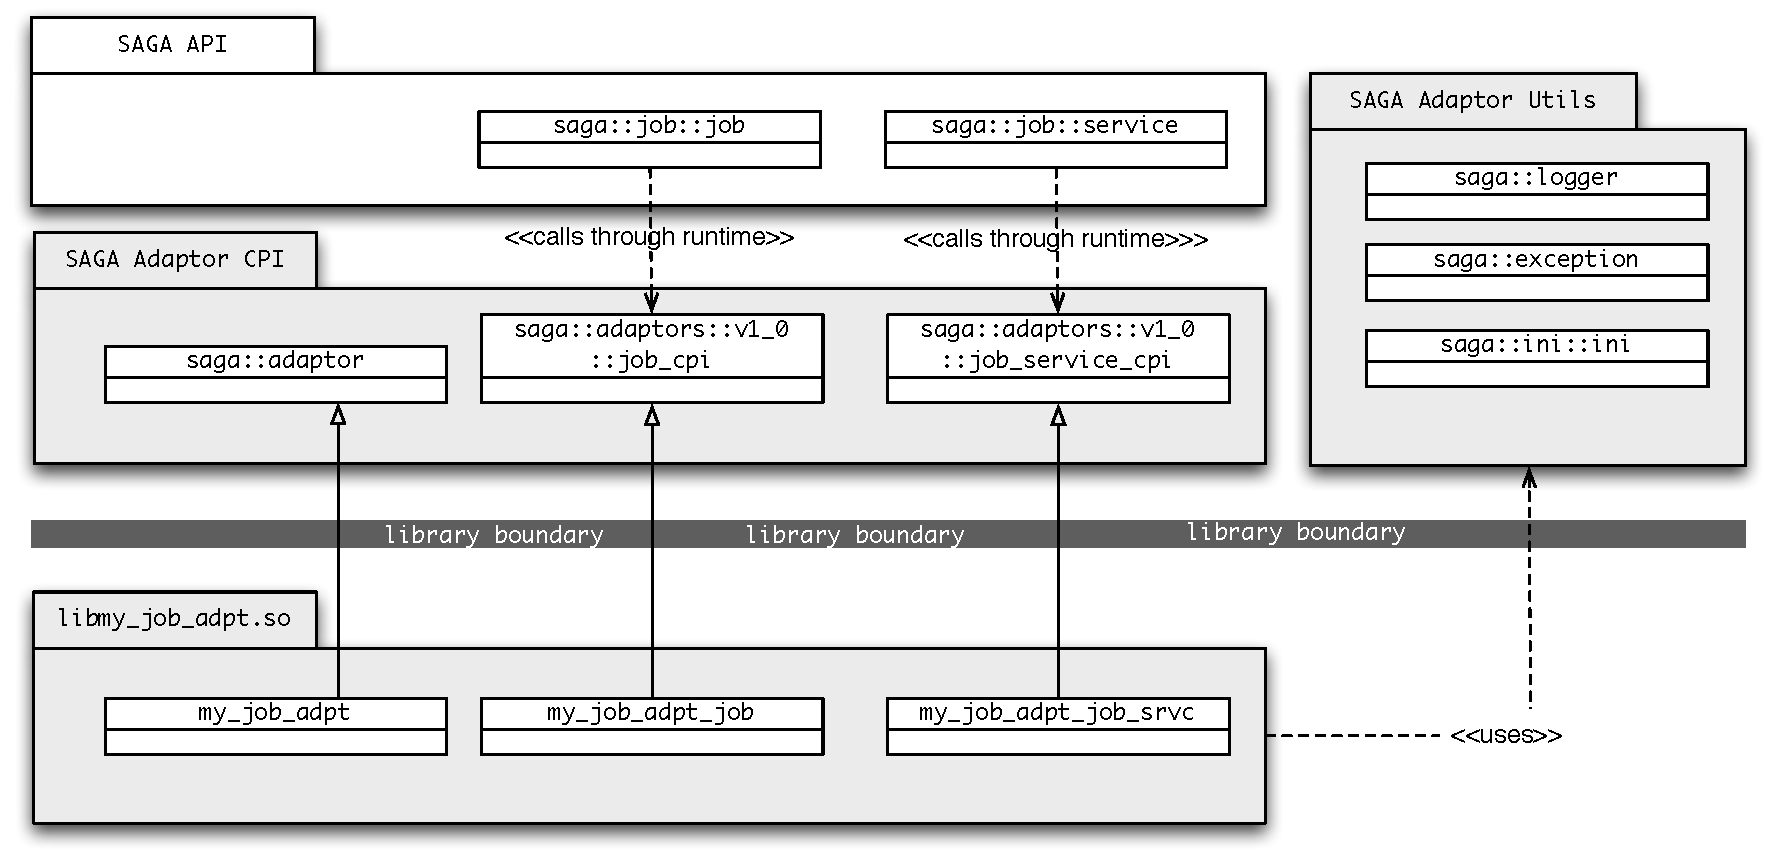
\includegraphics[scale=0.5]{figures/cpi-detail}
 \end{center}
 \caption{TODO}
\label{fig:cpi-detail}
\end{figure}

 
 \onote{Mention instancedata, adaptordata, ...}
 
 \subsubsection{Adaptors for Task Execution and Management}
 The various job adaptors obviously \textbf{O.W}
 
 \subsubsection{Adaptors for Data Access and Management}
 In the wake of a new important class of distributed applications that focus on 
 complex - often sensor-driven - data-intensive scientific workflows, data 
 management and access capabilities are becoming incresingly important for 
 application developers. Although SAGA does not provide a high-level abstraction
 for \textit{data} per se, it provides several functional packages that allow 
 and simplify low-level data access. These package APIs can easily be used to 
 develop a data abstraction framework on-top-of SAGA. The following list gives an
 overview of functional packages and adaptors that support data access and 
 management:
 
 \begin{itemize}

\item \textbf{File Package} - \onote{Short Description}

\begin{itemize}
\item Globus GridFTP File Adaptor
\item HDFS File Adaptor
\item Local File Adaptor
\item SSH File Adaptor

\end{itemize}

\item \textbf{Advert Package} - \onote{Short Description}

\begin{itemize}
\item PostgreSQL Advert Adaptor
\item SQLite3 Advert Adaptor
\end{itemize}

\item \textbf{Replica Package} - \onote{Short Description}

\begin{itemize}
\item PostgreSQL/SQLite3 Replica Adaptor
\item Globus RLS Replica Adaptor
\end{itemize}

\item \textbf{Stream Package}

\begin{itemize}
\item TCP Socket Stream Adaptor
\end{itemize}

\end{itemize}
 
 %This can (should)  include data as well as advert and replica adaptors \textbf{O.W}

 \subsubsection{Adaptors Bindings}
 Whatever else is worth mentioning: streams, sd, ... \textbf{O.W}


 \subsection{Python Language Bindings}
 \textbf{H.K., O.W}
 
 
 
 
 \subsection{Performance Aspects}
 T.B.D. (Look at old Globus adaptor benchmarks, etc..) \textbf{O.W}

 \subsection{Development Process}
 software architecture and development process and how it is designed to encourage and facilitate community contribution \textbf{O.W}


\section{Using SAGA: Applications, Tools and Frameworks} \textbf{S.J.}

 \subsection{Applications}
 \subsection{Tools}
 \subsection{Frameworks}

 
\section{Related Work}
 \textbf{S.J., O.W.}

\subsection{API for Distributed Functionality}

\subsection{Workflow Engines}

\section{Conclusion and Future Directions}

\section{Acknowledgements}
 
I'd like to thank Santa Claus for giving me my first computer. I'd also like 
to thank Baton Rouge for being such a crappy place that there is nothing other
than work to do out here, hence contributing immensely to the SAGA project :) 


 \bibliographystyle{IEEEtran} 
 \bibliography{the_saga_paper_abstract,saga_ogf}


\end{document}

